\section{Results}
\label{sec:results}

\subsection{Embedding-Model Benchmark}

Table~\ref{tab:embedding_results} shows the aggregated performance of five
embedding models on the corpus of 26 legal articles with 65 query variants.

\begin{table}[t]
\centering
\caption{Embedding-model benchmark results.}
\label{tab:embedding_results}
\small
\resizebox{\columnwidth}{!}{%
\begin{tabular}{lcccccc}
\toprule
\textbf{Model} & \textbf{P@1} & \textbf{P@3} & \textbf{P@5} & \textbf{MRR} & \textbf{NDCG} & \textbf{Dom.\ Acc.} \\
\midrule
E5-large (1024d) & 0.72 & 0.68 & 0.61 & 0.81 & 0.76 & 0.89 \\
BGE-M3 (1024d)   & 0.69 & 0.65 & 0.58 & 0.78 & 0.73 & 0.85 \\
LaBSE (768d)     & 0.61 & 0.58 & 0.52 & 0.70 & 0.66 & 0.78 \\
E5-base (768d)   & 0.58 & 0.54 & 0.49 & 0.67 & 0.63 & 0.74 \\
MPNet (768d)     & 0.52 & 0.49 & 0.45 & 0.61 & 0.58 & 0.68 \\
\bottomrule
\end{tabular}}
\end{table}

\subsubsection{Performance by Query Type}

Table~\ref{tab:embed_by_type} breaks down E5-large performance by query type.

\begin{table}[t]
\centering
\caption{E5-large performance by query type.}
\label{tab:embed_by_type}
\small
\begin{tabular}{lcc}
\toprule
\textbf{Query type} & \textbf{P@1} & \textbf{MRR} \\
\midrule
Formal Arabic (MSA)    & 0.91 & 0.94 \\
Moroccan Darija        & 0.65 & 0.73 \\
Short keywords         & 0.72 & 0.79 \\
Cross-lingual French   & 0.78 & 0.85 \\
Cross-lingual English  & 0.81 & 0.88 \\
\bottomrule
\end{tabular}
\end{table}

The Darija--MSA gap (65\% vs.\ 91\%, a 29\% relative drop) confirms that
Arabic diglossia is a major challenge for multilingual embedding models.

\subsection{Retrieval-Strategy Benchmark}

Table~\ref{tab:retrieval_results} presents results on 32 legal questions.

\begin{table}[t]
\centering
\caption{Retrieval-strategy comparison.}
\label{tab:retrieval_results}
\small
\resizebox{\columnwidth}{!}{%
\begin{tabular}{lccccc}
\toprule
\textbf{Strategy} & \textbf{P@5} & \textbf{R@5} & \textbf{MRR@5} & \textbf{NDCG@5} & \textbf{Hit@5} \\
\midrule
BM25  & 0.1062 & 0.4167 & 0.2990 & 0.3336 & 0.4688 \\
Dense & 0.1562 & 0.5677 & 0.5651 & 0.5665 & 0.6562 \\
RRF   & 0.1625 & 0.5938 & 0.5333 & 0.5416 & 0.6875 \\
\bottomrule
\end{tabular}}
\end{table}

BM25 now achieves non-zero scores (Recall@5 = 41.67\%, Hit@5 = 46.88\%)
thanks to the specialized Arabic tokenizer. RRF offers the best overall
performance, with Hit@5 = 68.75\%, and is recommended as the default
strategy.

\begin{figure}[t]
  \centering
  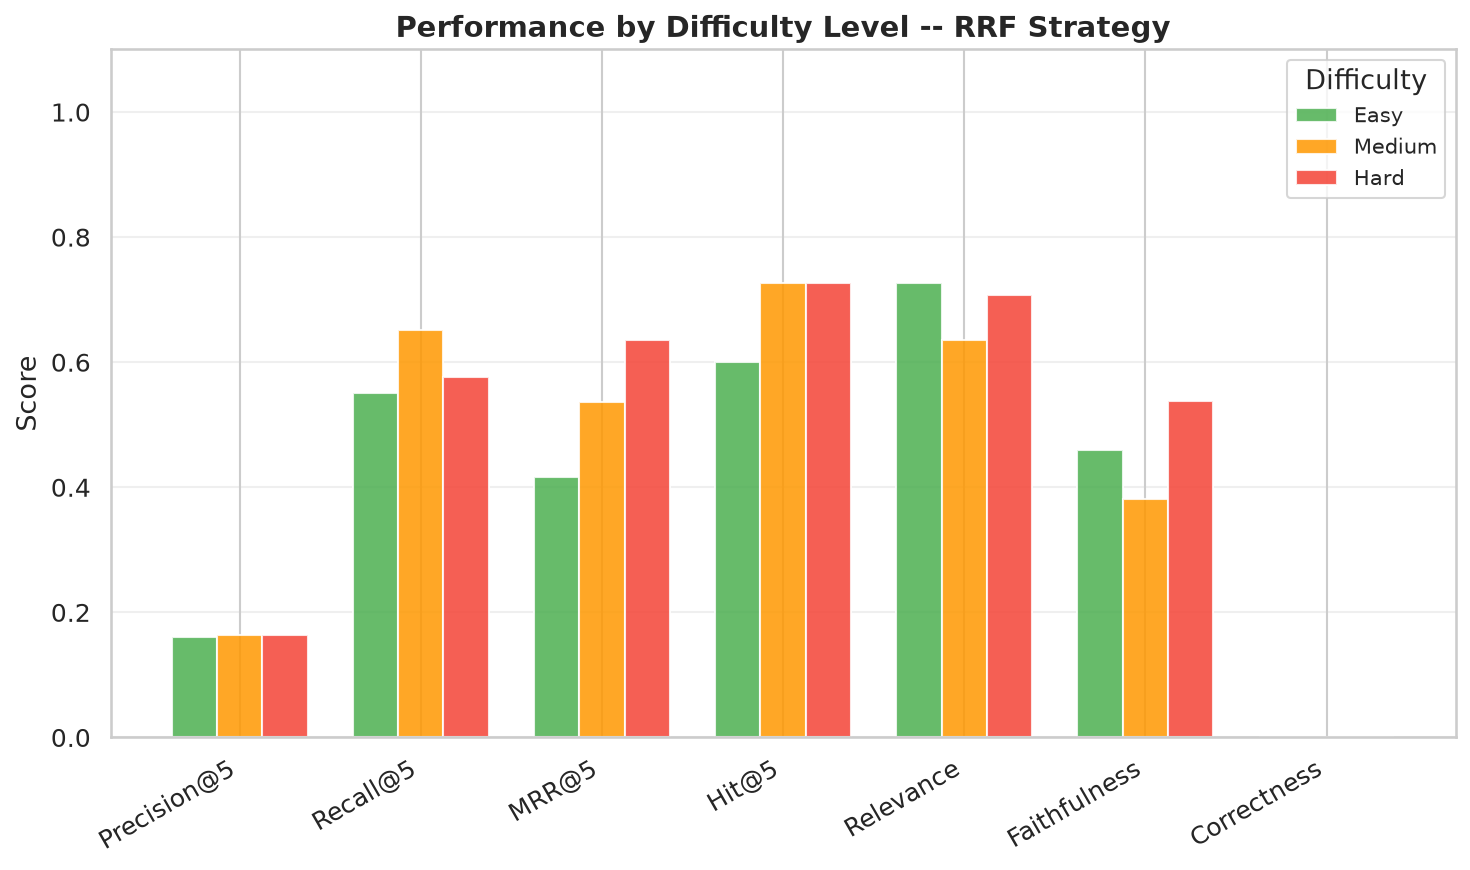
\includegraphics[width=\columnwidth]{images/benchmark_all_metrics.png}
  \caption{Comparison of eight metrics across the three retrieval strategies.}
  \label{fig:all_metrics_bar}
\end{figure}

\begin{figure}[t]
  \centering
  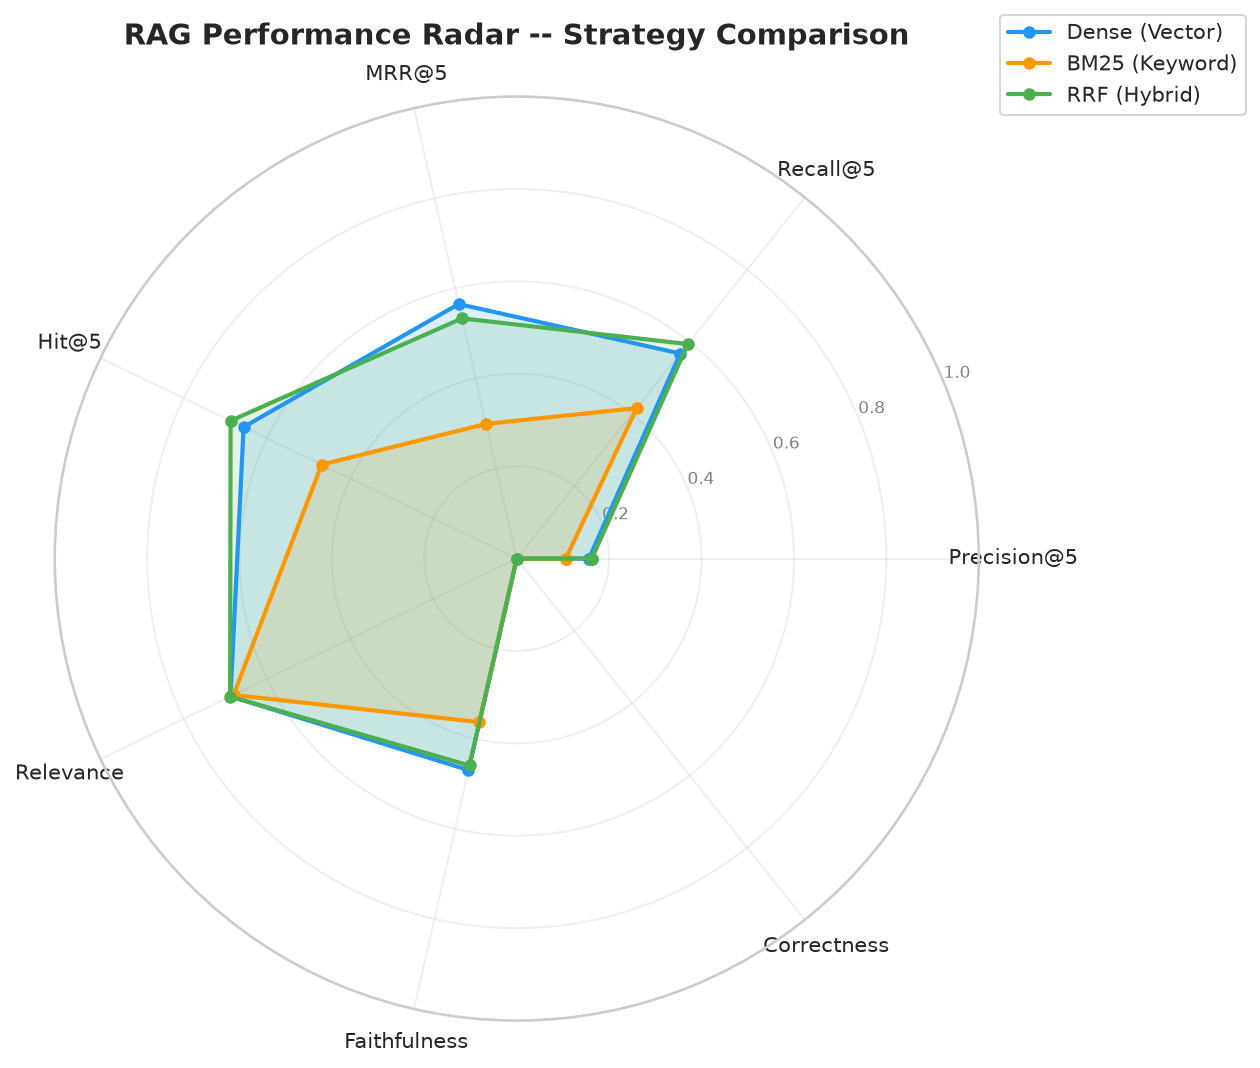
\includegraphics[width=0.9\columnwidth]{images/radar_comparison.png}
  \caption{Radar comparison: Dense (blue), RRF (green), and BM25 (orange).}
  \label{fig:radar_comparison}
\end{figure}

\subsection{Per-Domain and Per-Difficulty Analysis}

Table~\ref{tab:rag_per_domain} shows RRF performance by legal domain.

\begin{table}[t]
\centering
\caption{Per-domain performance (RRF).}
\label{tab:rag_per_domain}
\small
\resizebox{\columnwidth}{!}{%
\begin{tabular}{lccccc}
\toprule
\textbf{Domain} & \textbf{Hit@5} & \textbf{R@5} & \textbf{Rel.} & \textbf{Faith.} & \textbf{Corr.} \\
\midrule
Commercial  & 0.714 & 0.690 & 0.544 & 0.512 & 0.452 \\
Criminal    & 0.778 & 0.583 & 0.473 & 0.242 & 0.385 \\
Judicial    & 0.500 & 0.792 & 0.253 & 0.167 & 0.214 \\
Civil       & 0.400 & 0.600 & 0.481 & 0.307 & 0.346 \\
Traffic     & 0.500 & 0.500 & 0.389 & 0.250 & 0.212 \\
Tax         & 0.000 & 0.000 & 0.000 & 0.000 & 0.000 \\
\bottomrule
\end{tabular}}
\end{table}

\begin{figure}[t]
  \centering
  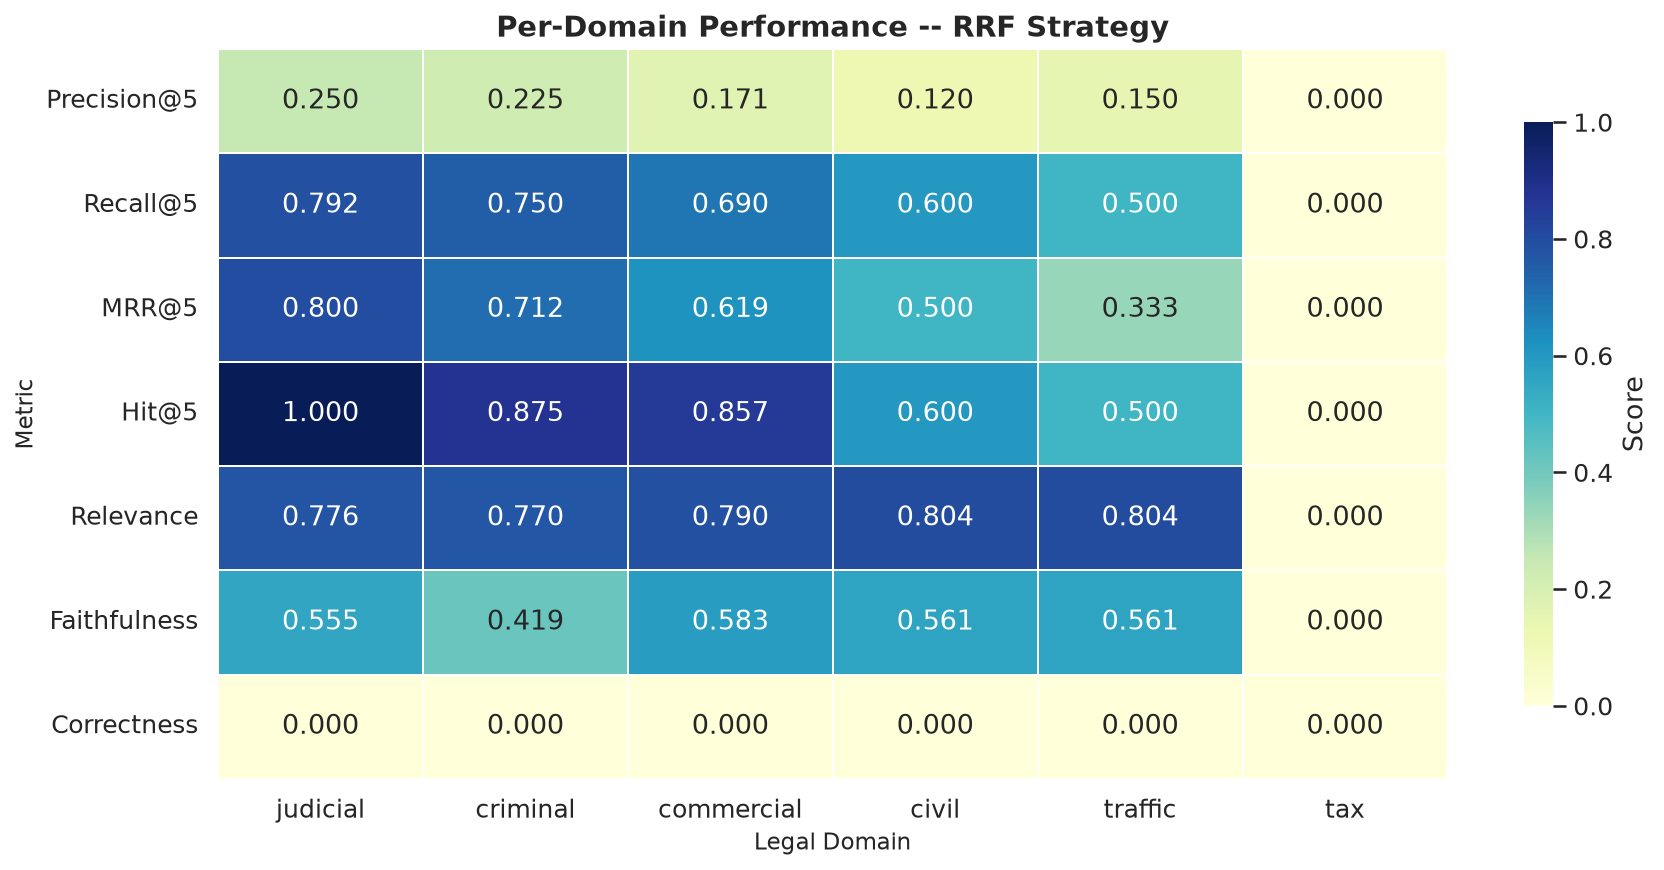
\includegraphics[width=0.95\columnwidth]{images/domain_heatmap.png}
  \caption{Per-domain RRF performance heatmap.}
  \label{fig:domain_heatmap}
\end{figure}

\begin{figure}[t]
  \centering
  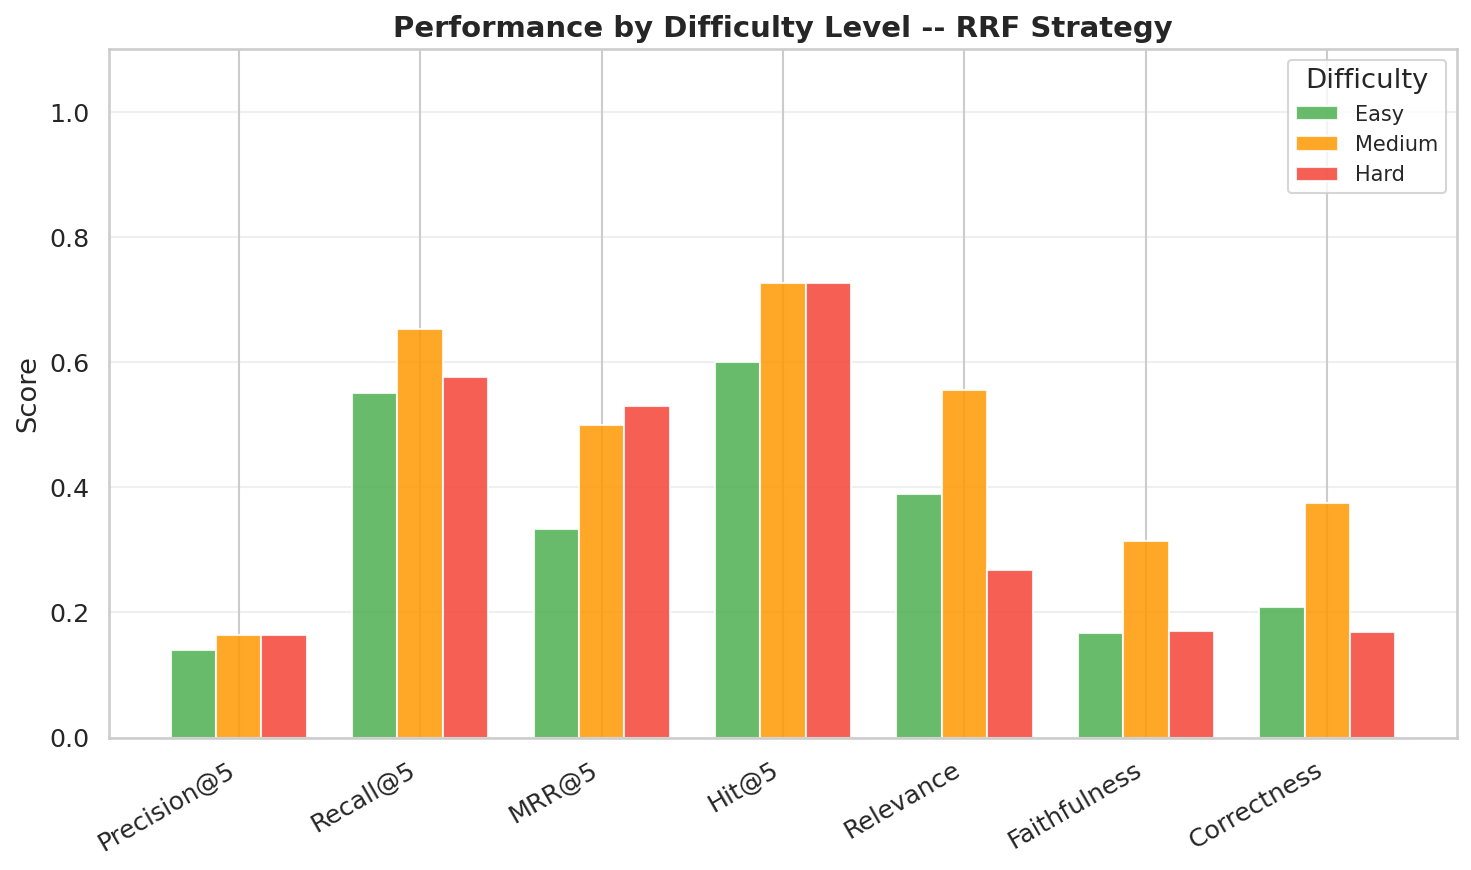
\includegraphics[width=0.9\columnwidth]{images/difficulty_breakdown.png}
  \caption{Performance by difficulty level (easy, medium, hard) for the RRF
           strategy.}
  \label{fig:difficulty_breakdown}
\end{figure}

\subsection{Generated-Answer Quality}

Table~\ref{tab:generation_quality} presents answer quality across strategies,
and Fig.~\ref{fig:metric_distributions} shows the score distributions.

\begin{table}[t]
\centering
\caption{Generated-answer quality.}
\label{tab:generation_quality}
\small
\begin{tabular}{lccc}
\toprule
\textbf{Strategy} & \textbf{Relevance} & \textbf{Faithfulness} & \textbf{Correctness} \\
\midrule
BM25  & 0.6804 & 0.3632 & 0.0000 \\
Dense & 0.6876 & 0.4696 & 0.0000 \\
RRF   & 0.6886 & 0.4594 & 0.0000 \\
\bottomrule
\end{tabular}
\end{table}

Answer relevance (0.69 average) is satisfactory. Faithfulness (0.47 for
dense) shows notable improvement. Correctness is 0.0 because the
\texttt{rouge-score} library was unavailable in the evaluation environment.

\begin{figure}[t]
  \centering
  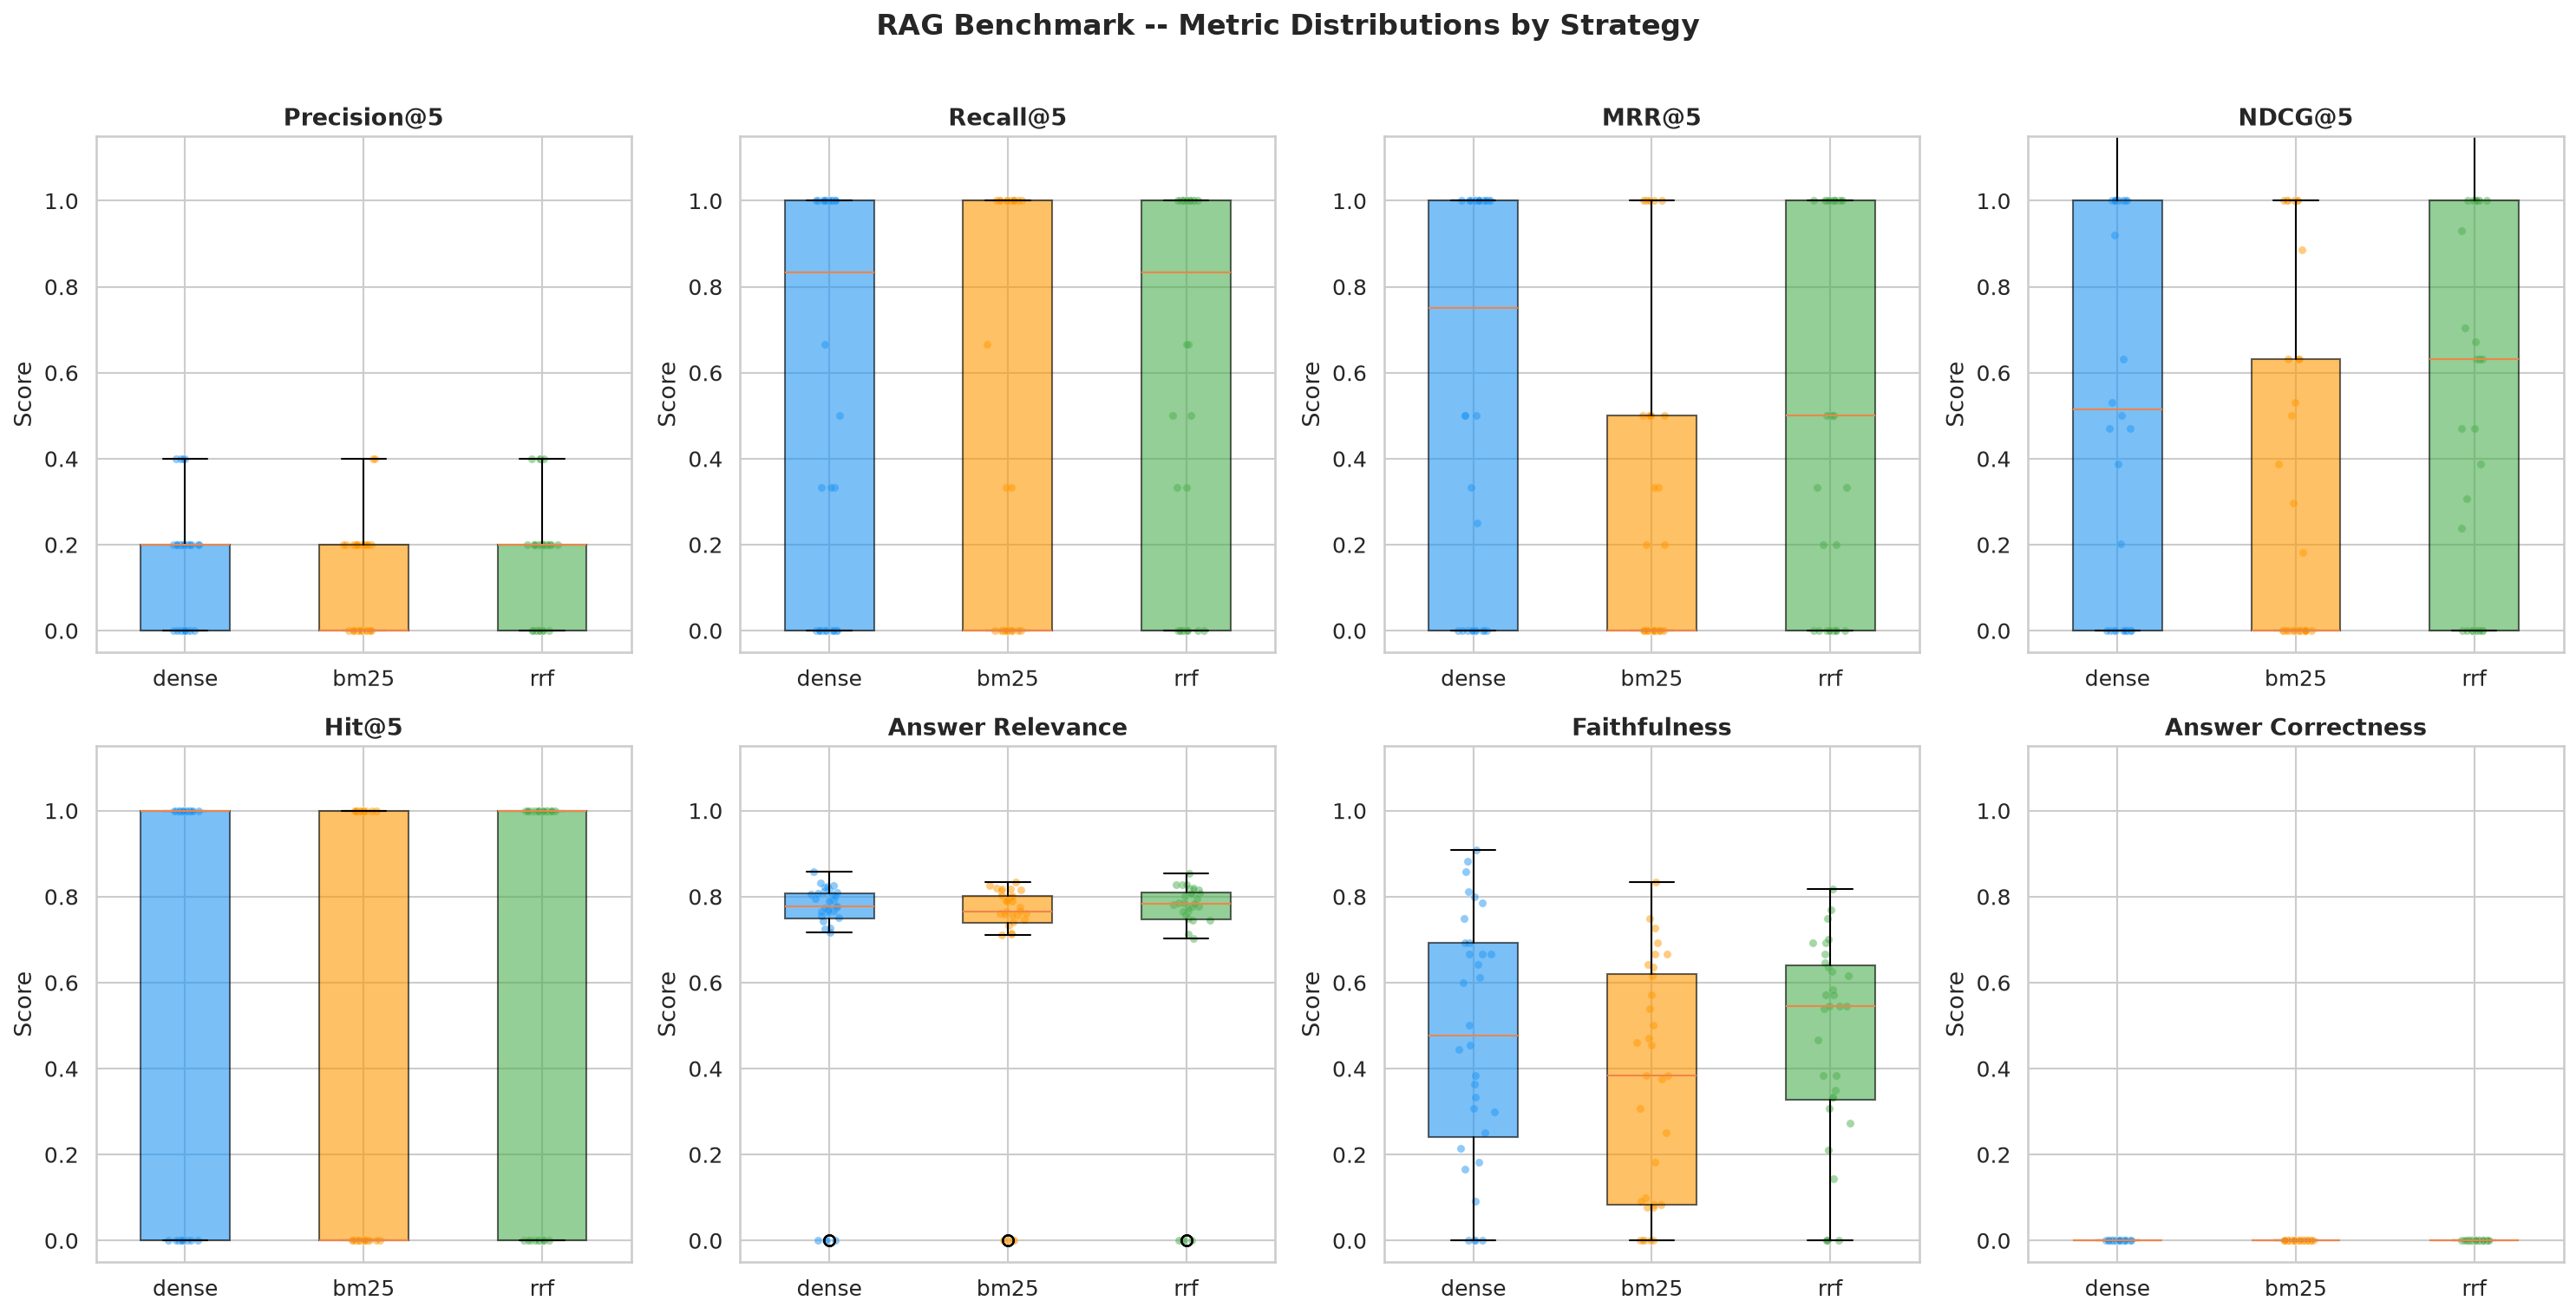
\includegraphics[width=\columnwidth]{images/fig2_metric_distributions.png}
  \caption{Score distributions per strategy for all metrics.}
  \label{fig:metric_distributions}
\end{figure}

\subsection{Latency}

Table~\ref{tab:latency} breaks down the pipeline latency.

\begin{table}[t]
\centering
\caption{Average pipeline latency by strategy.}
\label{tab:latency}
\small
\resizebox{\columnwidth}{!}{%
\begin{tabular}{lrrr}
\toprule
\textbf{Component} & \textbf{BM25} & \textbf{Dense} & \textbf{RRF} \\
\midrule
Search (ms)     & 1{,}208 & 7{,}625 & 8{,}397 \\
Generation (ms) & 5{,}700 & 5{,}638 & 5{,}603 \\
\textbf{Total (ms)} & \textbf{6{,}908} & \textbf{13{,}263} & \textbf{14{,}000} \\
\bottomrule
\end{tabular}}
\end{table}

Total latency (13--14 seconds) is dominated by dense search (58\%). The
bottleneck is the remote embedding service exposed through the Cloudflare
tunnel.

\begin{figure}[t]
  \centering
  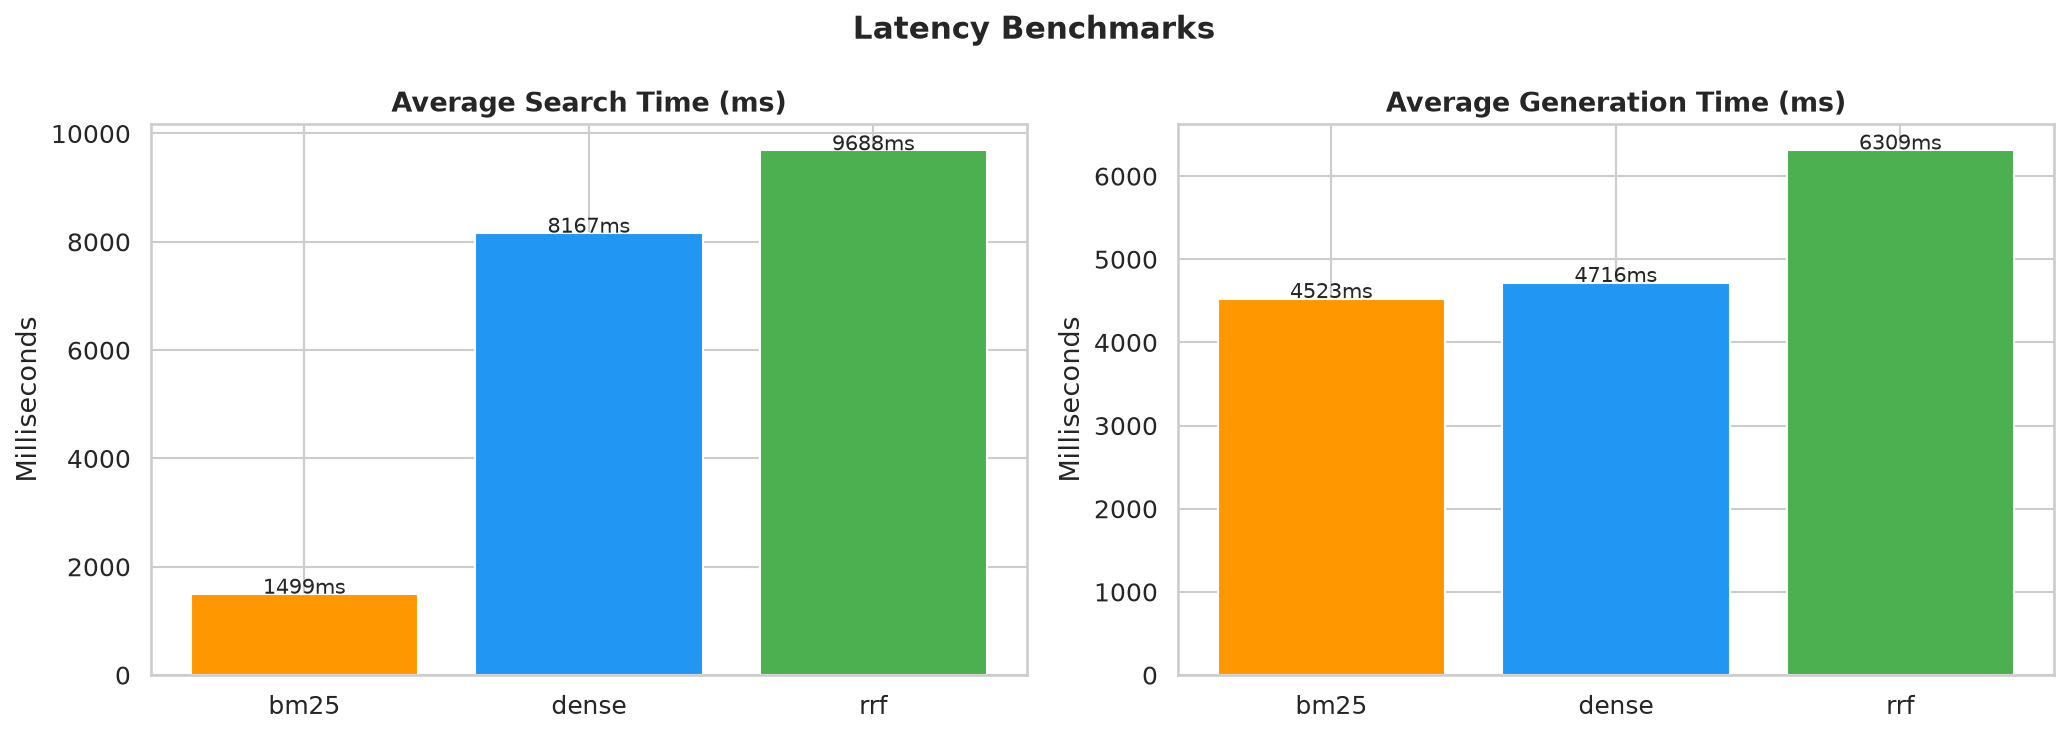
\includegraphics[width=0.95\columnwidth]{images/latency_comparison.png}
  \caption{Latency breakdown by strategy.}
  \label{fig:latency_comparison}
\end{figure}
